\documentclass[aspectratio=169,t]{beamer}
\usepackage[utf8]{inputenc}
\usepackage[T1]{fontenc}
\usepackage[english]{babel}
\usepackage{hyperref}
\usepackage{tikz}

\usepackage{graphicx}
\usepackage{epstopdf}
\usepackage{multirow}

\usepackage{psfrag}
\usepackage{pgfplots}
\usepackage{framed}
\usepackage{xcolor}
\usepackage{booktabs}
\usepackage{caption}
\usepackage{epstopdf}
\usepackage{amsmath}
\usepackage{tabularx}
\usepackage[]{bookmark}
%\usepackage[3D]{movie15}
%\usepackage{media9}
\usepackage[binary-units,abbreviations]{siunitx}
\usepackage[textfont=normalsize, labelfont=normalsize, justification=centering]{subcaption}
\usepackage{marvosym}
\usepackage{calc}
\usepackage{color, colortbl}
\usepackage[]{svg} 
\usepackage[]{trfsigns} 
\usepackage[nomessages]{fp}
\usepackage[]{csquotes}\MakeOuterQuote{"}
\selectcolormodel{rgb}

\makeatletter
\def\beamer@calltheme#1#2#3{\def\beamer@themelist{#2}
	\@for\beamer@themename:=\beamer@themelist\do
	{\usepackage[{#1}]{\beamer@themelocation/#3\beamer@themename}}}
\def\usefolder#1{\def\beamer@themelocation{#1}}
\def\beamer@themelocation{}
\usefolder{theme}

\usetikzlibrary{matrix,
	decorations.pathreplacing,
	calc,
	positioning,
	external,
	3d,
	shapes,
	arrows,
	pgfplots.statistics}
\pgfplotsset{compat=1.16}
\tikzstyle{faunode}=[rounded corners, draw=faublue, fill=faublue!10,  align=center, inner sep=0.3cm, line width=0.4mm]
\tikzstyle{fauellipseFixedWidth}=[ellipse, draw=faublue, fill=faublue!10,  align=center, inner sep=0.3cm, line width=0.4mm, minimum width=3cm]
\tikzstyle{fauellipse}=[ellipse, draw=faublue, fill=faublue!10,  align=center, inner sep=0.3cm, line width=0.4mm]
\tikzstyle{fauarrow}=[draw=faublue,->, line width=0.4mm]
\tikzstyle{fauline}=[draw=faublue, line width=0.4mm]


\usepackage[backend=bibtex,sorting=none,doi=true,style=phys]{biblatex}
%\usepackage[]{biblatex}
\bibliography{./references}

% Themes:
%  - fau:          FAU theme
%  - fau-tf:       TechFak FAU theme
%  - fau-tf-lme:   TechFak LME FAU theme
%
% Options:
%  - image:        Cover image on title page
%  - plain:        Plain title page
%  - longtitle:    Title page layout for long title
\usetheme[longtitle]{fau-tf-lme}

% END of THEME SETTINGS
% --------------------------------------------------------------------------------------------------------------------------------------------------------------------------

\sisetup{
exponent-product =\ensuremath{{\,\cdot\,}}
}

% Enable semi-transparent animation preview
\setbeamercovered{transparent}
\setbeamertemplate{blocks}[rounded]
\captionsetup{labelformat=empty,labelsep=none, labelfont=normalsize, justification=centering}


\newcommand\Wider[2][1.0cm]{%
\makebox[\linewidth][c]{%
  \begin{minipage}{\dimexpr\textwidth+#1\relax}
  \raggedright#2
  \end{minipage}%
  }%
}


\let\origitem\item
\renewcommand{\item}{\normalfont\origitem}
\newcommand{\bluefat}[1]{\textcolor{faublue}{\textbf{#1}}}
\newcommand{\bolditem}{\normalfont\origitem\bfseries}
\newcommand{\question}{{\bf Question: }}
\newcommand{\answer}{{\bf Answer: }}
\newcommand{\myExample}{{\bf Example }}
\newcommand{\real}{\mbox{${\mathbb R}$}}
\definecolor{defColor}{rgb}{0.8,0.87,0.97}
\definecolor{defColorT}{rgb}{0,0,0}
\definecolor{defColorF}{rgb}{1,1,1}
\newenvironment{myDefinition}{%
	\def\FrameCommand{\fboxsep=\FrameSep{} \fcolorbox{defColorF}{defColor}}%
	\color{defColorT}\MakeFramed{\FrameRestore{}}}%
{\endMakeFramed}

% Title page
\title[Medical Engineering II]{Medical Engineering - Imaging Systems}
\author{Prof.\ Dr.-Ing.\ habil.\ Andreas Maier}
\date{SS 2021}
\institute{Pattern Recognition Lab (CS 5)}

\newcommand{\password}{\texttt{mt2\_ss21}}


\AtBeginSection[]{
	{
		\setbeamertemplate{footline}{}
		\begin{frame}[noframenumbering]{\insertsubtitle}
			 \tableofcontents[currentsection]
		\end{frame} 
	}
}
\AtBeginSubsection[]{
	{

		\setbeamertemplate{footline}{}
		\begin{frame}[noframenumbering]{\insertsubtitle}
			 \tableofcontents[currentsection, currentsubsection]
		\end{frame} 
	}
}


%\usepackage[]{subfig} 
%\setbeamerfont{caption}{size=\Large}

\subtitle{X-Ray}
%\let\origitem\item
%\renewcommand{\item}{\normalfont\origitem}

\begin{document}

\subtitle{X-Ray}
\frame[plain,c]{\titlepage} % plain-Option deaktiviert Kopf- und Fusszeile


%subtitle
%toc for this chapter


\section{X-Ray History}

\begin{frame}{X-Ray History}
    \begin{itemize}
        \item November 8, 1895: Wilhelm Conrad Röntgen discovers X-rays
        \item December 28, 1895: Röntgen publishes the paper ``Über eine neue Art von Strahlen'' (On A New Kind Of Rays)
    \end{itemize}
    %
    \begin{figure}[tb]%
        \centering
        \begin{minipage}[t]{0.207\columnwidth}
            \includegraphics[width=1\columnwidth]{images/WilhelmRoentgen}%
            \caption{Wilhelm Conrad Röntgen}%
            \label{fig_chap:xray_roentgenHead}
        \end{minipage}
        \hspace{3cm}
        \begin{minipage}[t]{0.1998\columnwidth}
            \includegraphics[width=1\columnwidth]{images/EarlyXrayWife}%
            \caption{X-ray of his wife's hand.}%
            \label{fig_chap:xray_roentgenHand}
        \end{minipage}%
    \end{figure}
    %
    \begin{center}
        \vspace{-0.3cm}
        \begin{flushright}
            \scriptsize Sources: Wikimedia Commons
        \end{flushright}
    \end{center}
\end{frame}

\begin{frame}{Modern X-Ray Images}
    \begin{figure}
        \centering
        \begin{minipage}[t]{0.27\columnwidth}
            \includegraphics[height=0.7\textheight]{Siemens_Images/breastSmall}%
            \caption{Breast X-ray. Note the clearly visible structures in the soft-tissue.}
            \label{fig_chap:xray_breastExample}
        \end{minipage}
        \hspace{2cm}
        \begin{minipage}[t]{0.415\columnwidth}
            \includegraphics[height=0.7\textheight]{Siemens_Images/150_7}%
            \caption{X-ray taken from the thorax (chest) of a patient.}
            \label{fig_chap:xray_CTexample}
        \end{minipage}%
    \end{figure}
    \vspace{-0.5cm}
    \begin{flushright}
        \scriptsize Sources: Siemens Healthcare, Erlangen, Germany
    \end{flushright}
\end{frame}

\begin{frame}{Nature of X-Rays}
    \begin{center}\vspace{0cm}
        \includegraphics[width=0.9\columnwidth]{images/wavelengthFrequ}%
    \end{center}\vspace{-0.1cm}
    \begin{itemize}
        \item X-rays belong to the group of electromagnetic radiation
        \item Characterized by wavelength $\lambda_p$ or frequency $f_p$, where $\lambda_p=c_0/f_p$
        \item Typical wavelengths for X-rays: $10^{-8}$ to $10^{-11}$ m
    \end{itemize}
\end{frame}

\begin{frame}{Nature of X-Rays}
    \begin{itemize}
        \item Energy of X-rays is also determined by their wavelength
              \begin{equation*}
                  E_p = \frac{h c_0}{\lambda_p} = h f_p
              \end{equation*}
      \item {$h$ denotes Planck's constant, with $h\ \approx\SI{6.626069d-34}{\joule\second}$}\\
        \item {The energy unit is electron volt [eV]}
        \item {1eV is the kinetic energy that a particle with the charge of an electron achieves when being accelerated in a potential difference of 1V}
    \end{itemize}
\end{frame}

\begin{frame}{Nature of X-Rays}
    \textbf{Absorption of X-rays}
    \begin{itemize}
        \setlength\itemsep{0.2cm}
        \item X-ray photons are partially absorbed while traveling through the patient. This process is also called attenuation.
        \item Attenuation is higher in dense materials than in non-dense materials
        \item This difference in attenuation leads to contrast in the image
        \item E.\,g.\ bones appear darker than soft tissue as more photons are absorbed
        \item The amount of attenuation also depends on the energy of the X-rays
    \end{itemize}
\end{frame}


\begin{frame}{Nature of X-Rays}
    \textbf{Propagation of X-rays}
    \begin{itemize}
        \item X-rays are propagated along straight lines through homogeneous material
    \end{itemize}
    \vspace{0.5cm}
    \textbf{Refraction of X-rays}
    \begin{itemize}
        \item Refraction is the change of direction at the transition of two different media
        \item Refraction of X-rays is very small, thus building X-ray lenses is an open problem
    \end{itemize}
    \vspace{0.5cm}
    \textbf{Diffraction of X-rays}
    \begin{itemize}
        \item X-rays are slightly bent when passing an edge or slit
        \item Exploited in \emph{Phase Contrast Imaging}
    \end{itemize}
\end{frame}

%\begin{frame}{Energy of a Photon}
%\begin{itemize}
%\item {\bf 1 eV (1 electron volt): }\\
%kinetic energy that a charged particle of one elementary charge (i.e. charge of an electron)
%achieves while being accelerated in a potential difference of 1V.
%\item If the anode voltage is 100 kV, each electron gets a kinetic energy of
%\begin{eqnarray} 100 \ keV = 100 \cdot 10^3 \ eV \end{eqnarray}
%\end{itemize}
%\end{frame}


%\begin{frame}
%{Energy of a Photon}
%The energy $E_{photo}$ of a photon is given by:
%\begin{eqnarray}
%E_{photo}&=&\hbar\cdot \nu
%\end{eqnarray}
%where $\nu$ denotes the frequency of electromagnetic radiation and $\hbar$ is
%Planck's constant:
%$$
%\hbar= 6.62606957 \cdot 10^{-34} \quad \frac{m^2 kg}{s}.
%$$
%\end{frame}

%\begin{frame}
%{Kinetic Energy of an Electron}

%The kinetic energy $E_{kin}$ of an electron is given by:
%\begin{eqnarray}
%E_{kin}&=&e \cdot U_A
%\end{eqnarray}

%where $e$ is the electron charge and
%$U_A$ the voltage at the anode.
%\end{frame}

%\begin{frame}{Minimum Wavelength}
%\begin{itemize}
%\item If the kinetic energy of the electron is completely converted into the energy of a photon,
%the following equation holds:
%\begin{eqnarray}
%E_{kin}         &=& E_{photo} \quad=\quad
%e \cdot U_A \quad=\quad \hbar\cdot \nu	\nonumber
%\end{eqnarray}
%\item This identity can be used to compute the maximum frequency of the resulting photon:
%\begin{eqnarray}
%\nu_{\max} &=& \frac{e \cdot U_A} {\hbar}
%\end{eqnarray}
%\item The minimum wavelength results from the fact that the product of wavelength and frequency is the speed
%of light, i.e. $c= \lambda \nu$:
%\begin{eqnarray}
%\lambda_{min} &=& \frac{c}{\nu_{\max}}\quad=\quad\frac{c \cdot \hbar}{e \cdot U_A}
%\end{eqnarray}
%\end{itemize}

%\end{frame}
%
%
%%%%%%%%%%%%%%%%%%%%%%%%%%%%%%%%%%%%%%%%%%%%%%%%%%%%%%%%%%%%%%%%%%%%%%%%%%%%%%%%%%%%%%%%%%%
%%% Section X-ray Generation
% 
% 

\section{Generation of X-Rays}




\begin{frame}{Generation of X-Rays}
    \centering
    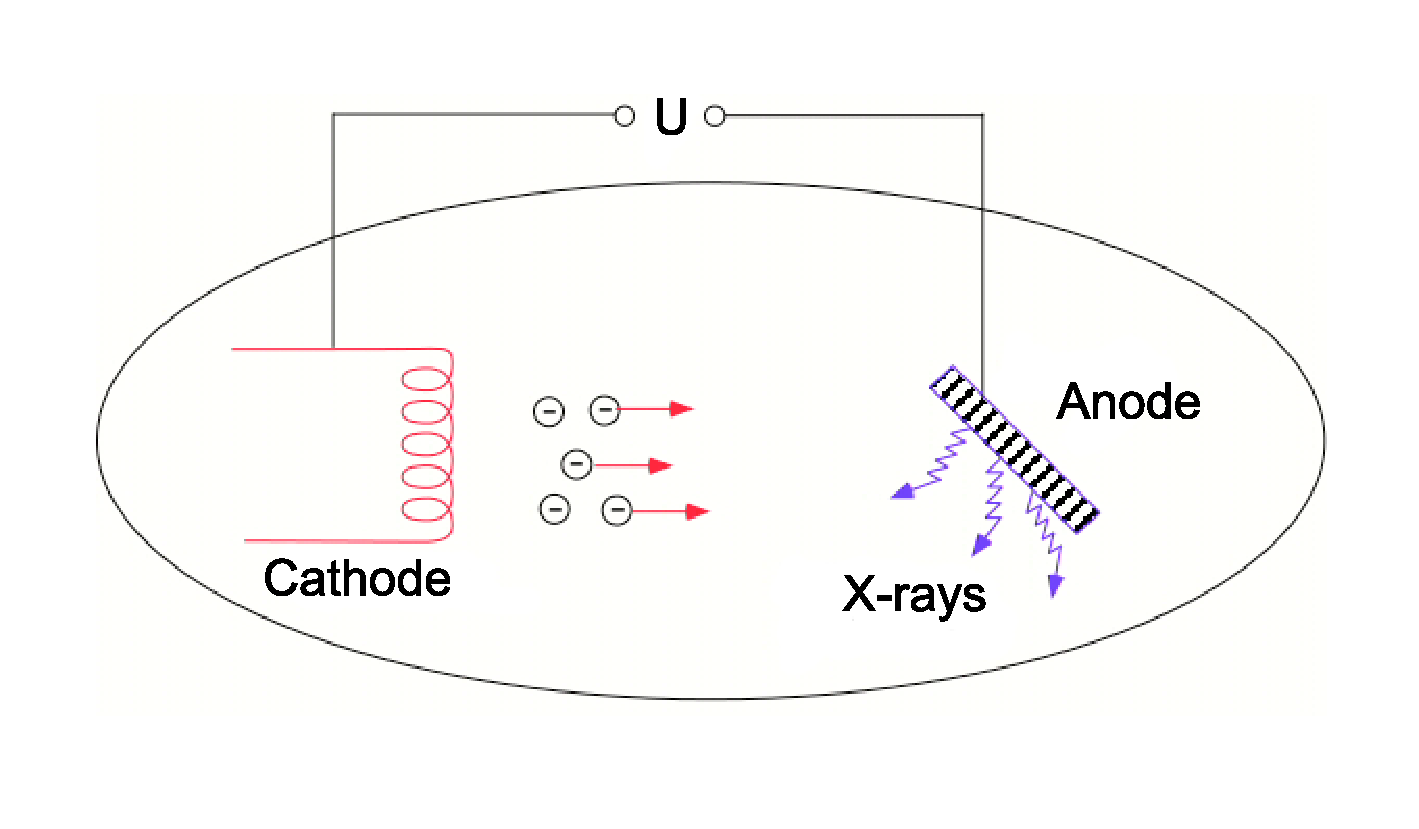
\includegraphics[height=0.7\textheight]{images/xraytube_closeup}\\
    \begin{itemize}
        \item X-ray tube current: when high potential difference is applied across the tube, electrons flow from cathode filament to anode
    \end{itemize}
\end{frame}

\begin{frame}{The Cathode}
    \begin{itemize}
        \item The cathode is the negative side of the tube. It consists of two principle parts:
              \begin{itemize}
                  \item The filaments: mostly two which provides large and small focal area
                  \item The focusing cup houses the filaments. Has negative voltage to focus the beam to a small area
              \end{itemize}

    \end{itemize}
    \centering
    \includegraphics[width=0.3\textwidth]{images/cathode}\\

\end{frame}

\begin{frame}[c]{The Anode}
    \begin{itemize}
        \item The anode is the positive side of the tube
        \item Can be classified by the type and usage:
              \begin{itemize}
                  \item Stationary: long exposure times, large focal spots. (dental X-ray)
                  \item Rotating: short exposure times, smaller focal spots with high resolution
              \end{itemize}

    \end{itemize}
    \centering
    \includegraphics[height=0.6\textheight]{images/x-ray_tube.jpg}\\[-0.5\baselineskip]
    {\tiny Source: Medical Imaging Systems: An introductory guide~\cite{Berger2018}}


\end{frame}


\begin{frame}[t]{Quality Aspects for Medical X-Ray Generators}
    \begin{itemize}
        \setlength\itemsep{0.4cm}
        \item High power $\longrightarrow$ short exposure time
        \item Small focus $\longrightarrow$ sharp images
        \item Variable photon energy $\longrightarrow$ contrast
        \item Cost efficient production
        \item Low service and long durability
    \end{itemize}
\end{frame}

\begin{frame}{Focal Spot Size}
    The focal spot size is the anode area that is hit by the electron beams

    \begin{itemize}
        \item Penumbra at X-ray Images
    \end{itemize}

    \begin{center}\includegraphics[height=0.7\textheight ]{images/penumbra}\end{center}
    \begin{flushright}
    \end{flushright}
\end{frame}

\begin{frame}[c]{Technical Aspects of a X-Ray Tube}
    \begin{columns}[c]
        \column{.4\textwidth}
        \begin{itemize}
            \item A modern rotating anode X-ray tube encased in a metal or glass protective housing
            \item It contains two principle parts: the rotating anode and the cathode
            \item Vacuum tube
        \end{itemize}
        \column{.5\textwidth}
        \includegraphics[width=\textwidth]{images/Rotating_anode_x-ray_tube_(labeled).jpg}

        \begin{flushright}
            \tiny Source: Daniel W. Rickey (CC BY-SA 3.0)
        \end{flushright}
    \end{columns}
\end{frame}



\begin{frame}{Cross-Sectional View of a Turning Anode Tube}
    \centering
    \includegraphics[height=0.65\textheight]{images/xraytube}\\
    \begin{itemize}
        \item Acceleration Voltage: 20 to 150 kV
        \item Electron Current: 1 to 5 mA (for continuous operation)
        \item Electron Current: 0.1 to 1.0 A (for short exposures)
    \end{itemize}

\end{frame}


%\begin{frame}{Solutions for \\Heat Problem}
%\vspace{-30mm}
%\begin{columns}
%\column{.4\textwidth}
%\vspace{-\textwidth}
%\begin{center}
%\begin{itemize}
%\item tilted anode
%\item rotating anode
%\end{itemize}
%\end{center}
%\column{.6\textwidth}
%%Todo: graphic ch1a_38
%\vspace{-25mm}
%\includegraphics[height=1\textheight]{images/ismd-7-9}\\[18mm]
%{\scriptsize \hskip24pt Source: Oppelt: Imaging Systems for Medical Diagnostics}
%\end{columns}
%\end{frame}

%\begin{frame}{Temperature of a Single Spot on the Anode Surface}
%\begin{center}\includegraphics[height=0.8\textheight ]{images/ch1a-40}\end{center}
%\begin{flushright}
%\scriptsize Source: Slides BVM
%\end{flushright}
%\end{frame}

%\begin{frame}{Selection Criteria for Anode Material}
%\begin{itemize}
%\item high atomic number $Z$ $(\eta = k \cdot U_A\cdot Z)$
%\item high melting point $T_{\max}$
%\item high thermal conductivity $\lambda$
%\item high specific heat capacity $c$
%\end{itemize}
%\vspace{5ex}
%Quality measure for fixed anodes: $ Z \cdot T_{\max} \cdot \lambda$\\
%Quality measure for turning anodes: $ Z \cdot T_{\max} \cdot \sqrt{\lambda\rho c}$
%\end{frame}

%\begin{frame}{Different Anode Materials and Their Suitability}
%\begin{center}
%\small
%\begin{tabular}{c|c|c|c|c|c|c|c|c|}
%\multirow{2}{*}{element} & \multirow{2}{*}{atomic number Z} & permissible temperature $T_{\max}$      & thermal conductivity                     & \multicolumn{2}{|c|}{fixed anode} & \multicolumn{3}{|c|}{turning anode}                                                                                  \\
%&                                  & at $1.33\cdot 10^{-2}$ Pa in $^\circ C$ & $\lambda$ $\left[\frac{W}{cm\ K}\right]$ & $Z\ T_{\max}\ \lambda$            & Rank                                & $\sqrt{\lambda\rho c}$ & $ Z \cdot T_{\max} \cdot \sqrt{\lambda\rho c}$ & rank \\
%\hline
%Cu                       & 29                               & 1,032                                   & 3.98                                     & 119,113                           & 8                                   & 3.68                   & 110,135                                        & 10   \\
%Mo                       & 42                               & 2,167                                   & 1.38                                     & 125,599                           & 7                                   & 1.88                   & 171,106                                        & 8    \\
%Ag                       & 47                               & 832                                     & 4.18                                     & 163,450                           & 4                                   & 3.18                   & 124,350                                        & 9    \\
%Ta                       & 73                               & 2,587                                   & 0,55                                     & 103,868                           & 9                                   & 1.13                   & 213,402                                        & 6    \\
%\hline
%W                        & 74                               & 2,757                                   & 1.3                                      & 265,223                           & 1                                   & 1.81                   & 369,273                                        & 1    \\
%\hline
%Re                       & 75                               & 2,557                                   & 0.71                                     & 136,160                           & 6                                   & 1.38                   & 264,650                                        & 4    \\
%Os                       & 76                               & 2,280                                   & 0.87                                     & 150,754                           & 5                                   & 1.77                   & 306,706                                        & 3    \\
%Ir                       & 77                               & 2,220                                   & 1.46                                     & 249,572                           & 3                                   & 2.06                   & 352,136                                        & 2    \\
%Pt                       & 78                               & 1,742                                   & 0.71                                     & 96,472                            & 10                                  & 1.41                   & 191,585                                        & 7    \\
%Au                       & 79                               & (1,063)                                 & 3.14                                     & 263,687                           & 2                                   & 2.81                   & 235,975                                        & 5    \\
%U                        & 92                               & (1,132)                                 & 0.25                                     & 26,036                            & 11                                  & 0.75                   & 78,108                                         & 11   \\
%\end{tabular}
%\end{center}
%\end{frame}

%\begin{frame}{Setup of a Turning Anode}
%\begin{center}\includegraphics[width=\textwidth ]{images/ch1b-2-1}\end{center}
%\begin{flushright}
%\scriptsize Source: Slides BVM
%\end{flushright}
%\end{frame}

%\begin{frame}{Double Angle Anode}
%\vspace{-0.2\textheight}
%\begin{center}\hspace{3ex}\includegraphics[height=1\textheight ]{images/ch1b-2-2}\end{center}
%\begin{flushright}
%\scriptsize Source: Slides BVM
%\end{flushright}
%\end{frame}

%%\begin{frame}{Sliding Contact Bearing}
%%%Todo: graphic ch1a_39
%%\vspace{0.1\textheight}
%%\begin{center}\includegraphics[widht=\textwidth ]{images/ch1a-47}\end{center}
%%\begin{flushright}
%%\scriptsize Source: Slides BVM
%%\end{flushright}
%%\end{frame}

%\begin{frame}{Anode Current Control}
%electrons are emitted by thermionic emission
%\[j_e = A_{0} T^2 \textnormal{e}^\frac{-W}{k\ T}\]
%\begin{table}[t]
%\centering
%\begin{tabular}{r l}
%$j_e$ & = emission current density             \\
%$A_0$ & = material constant                    \\
%$T$   & = temperature in Kelvin                \\
%$W$   & = work function, for tungsten = 4.5 eV \\
%$k$   & = Boltzmann constant                   \\
%\end{tabular}
%\end{table}
%anode current is controlled by heating current
%\end{frame}

%\begin{frame}{Dependency of Anode Voltage and Anode Current}
%%Todo: graphic ch1a_39
%\begin{center}\includegraphics[height=0.8\textheight ]{images/ch1a-50}\end{center}
%\begin{flushright}
%\scriptsize Source: Slides BVM
%\end{flushright}
%\end{frame}

%%\begin{frame}{12-Pulse Generator}
%%%Todo: graphic ch1a_39
%%\vspace{-0.15\textheight}
%%\begin{center}\includegraphics[height=1\textheight ]{images/ch1a-51}\end{center}
%%\begin{flushright}
%%\scriptsize Source: BVM
%%\end{flushright}
%%\end{frame}

%\begin{frame}{High-Frequency Generator}
%%Todo: graphic ch1a_39
%\begin{center}\includegraphics[width=\textwidth ]{images/ch1a-52}\end{center}
%\begin{flushright}
%\scriptsize Source: BVM
%\end{flushright}
%\end{frame}

%\begin{frame}{Exposure Control}
%%Todo: graphic ch1a_39
%emitted dose:
%\[ D_{tot}=k\cdot Z\cdot I_A\cdot U_A^2\cdot T \]

%\begin{tabular}{r l}
%$T$ & = exposure time \\
%\end{tabular}

%\vspace{5ex}
%image-producing dose:
%\[ D_{img}=k^* \cdot Z\cdot U^n \cdot I \cdot T \]
%\vspace{2ex}
%\begin{tabular}{r l}
%$k^*$ & = imaging system dependent parameter                                \\
%$n$   & = voltage dependent parameter, for $U=150 \text{ kV}$, $n\approx 3$
%\end{tabular}
%\end{frame}

%\begin{frame}{Exposure Control}
%\[ D_{img}=k^* \cdot Z\cdot U^n \cdot I \cdot T \]
%\begin{itemize}
%\item timing devices: $U\text{,} I$ and $T$ have to be selected
%\item 'mAs switching': $U$ and $Q=I\cdot T$ have to be selected
%\item automatic exposure control system: Only $U$ has to be selected
%\end{itemize}
%$\Longrightarrow$ automatic selection of current $I$ over time $T$\\[2\baselineskip]
%switching the tube on and off
%\begin{itemize}
%\item by changing the voltage $U$
%\item using a grid between anode and cathode
%\end{itemize}
%\end{frame}

%\begin{frame}{Generator Variations of Applied Dose}
%\begin{center}\includegraphics[height=0.8\textheight ]{images/ismd-12-39}\end{center}
%\begin{flushright}
%\vspace{-10mm}
%\scriptsize Source: Oppelt: Imaging Systems for Medical Diagnostics
%\end{flushright}
%\end{frame}

%\begin{frame}{Typical Load Curves}
%\vspace{-30mm}
%\begin{columns}
%\column{0.3\textwidth}
%\\
%\column{0.7\textwidth}
%\begin{center}\includegraphics[height=1\textheight ]{images/ch1b-9}\end{center}
%\end{columns}
%\begin{flushright}
%\vskip-5mm
%\scriptsize Source: Slides BVM
%\end{flushright}
%\end{frame}

%\begin{frame}{Generator with 'Falling Load'}
%\begin{center}\includegraphics[height=0.7\textheight ]{images/ch1b-10}\end{center}
%$\Longrightarrow$ shorter exposure time
%\begin{flushright}
%\scriptsize Source: Slides BVM
%\end{flushright}
%\end{frame}


\begin{frame}[c]{X-ray energy spectrum}

    Typical Values for X-Rays:
    \vspace{0.4cm}
    \begin{itemize}
        \setlength\itemsep{0.4cm}
        \item {\em soft X-rays}:
              \begin{itemize}
                  \item  $U_A$ up to  $1$ kV
                  \item $10$ to $1$ nm wavelength
              \end{itemize}
        \item {\em average X-rays}:
              \begin{itemize} \item $U_A$ up to  $10$ kV \end{itemize}
        \item {\em hard X-rays}:
              \begin{itemize}
                  \item $U_A$ from $10$ up to $120$ kV \\
                  \item $0.10$ to $0.01$ nm wavelength
              \end{itemize}
    \end{itemize}
\end{frame}


\begin{frame}{X-ray energy spectrum}
    The X-ray tube provides an environment for X-ray production via bremsstrahlung and characteristic radiation mechanisms.
    \vspace{-0.4cm}
    \begin{center}%
    \includegraphics[height=0.8\textheight, trim={0  0.0cm 0 0.5cm},clip]{images/spectrum_2types}
\end{center}
\end{frame}



%\begin{frame}{Bremsstrahlung}
%\begin{itemize}
%\setlength\itemsep{0.4cm}
%\item If an electron passes close to an atomic nucleus, it will most probably change its fly direction and undergoes an acceleration
%\item There is a small probability that the electron looses energy in the form of a photon while being deflected
%\item These photons are called bremsstrahlung photons and these photons are the basis for X-ray diagnostic imaging
%\item Bremsstrahlung photons can obtain an arbitrary energy between 0 and the complete kinetic energy of the electron
%\item Relative amount of bremsstrahlung emitted increases with increasing electron kinetic energy and with increasing atomic number, $Z$, of the anode material.
%\end{itemize}
%\end{frame}

\begin{frame}[c]{Bremsstrahlung}
    On the event of an electron passing close to an atomic nucleus\ldots

    \vspace{0.4cm}
    \begin{itemize}
        \setlength\itemsep{0.4cm}
        \item \bluefat{Probable Event:} acceleration and change of direction
        \item \bluefat{Less probable:} deceleration and generation of a photon
              \vspace{0.2cm}

              \begin{itemize}
                  \setlength\itemsep{0.2cm}
                  \item Conversion of kinetic energy to a photon:  \textit{Bremsstrahlung}
                  \item Bremsstrahlung photons can obtain an arbitrary energy between 0 and the complete kinetic energy of the electron
                  \item Relative amount of bremsstrahlung emitted increases with increasing electron kinetic energy and with increasing atomic number, $Z$, of the anode material.
              \end{itemize}
    \end{itemize}
    \vspace{0.4cm}

    Bremsstrahlung photons are the basis for X-ray diagnostic imaging
    %\begin{itemize}
    %\setlength\itemsep{0.4cm}
    %\item If an electron passes close to an atomic nucleus, it will most probably change its fly direction and undergoes an acceleration
    %\item There is a small probability that the electron looses energy in the form of a photon while being deflected

    %\begin{itemize}
    %\setlength\itemsep{0.3cm}
    %\item These photons are called bremsstrahlung photons and these photons are the basis for X-ray diagnostic imaging
    %\item Bremsstrahlung photons can obtain an arbitrary energy between 0 and the complete kinetic energy of the electron
    %\item Relative amount of bremsstrahlung emitted increases with increasing electron kinetic energy and with increasing atomic number, $Z$, of the anode material.
    %\end{itemize}
    %\end{itemize}
\end{frame}

% \begin{frame}{Spatial Distribution of Bremsstrahlung}
% \begin{center}\includegraphics[height=0.8\textheight ]{images/ch1a-13}\end{center}
% \begin{center}
% \scriptsize Source: BVM
% \end{center}
% \end{frame}
% 
% \begin{frame}{Distribution of X-Rays on Anode Surface}
% \begin{center}\includegraphics[width=0.7\textwidth ]{images/ch1a-14}\end{center}
% \begin{center}
% \scriptsize Source: Slides BVM
% \end{center}
% \end{frame}

%\iffalse
%\begin{frame}{Bremsstrahlung}
%\begin{columns}
%\column{.5\textwidth}
%\includegraphics[scale=.75]{images/ch1a-15-1}
%\column{.5\textwidth}
%\includegraphics[scale=.75]{images/ch1a-15-2}
%\end{columns}
%\begin{columns}
%\column{.5\textwidth}
%single interaction
%\column{.5\textwidth}
%several interactions in series
%\end{columns}
%\begin{flushright}
%\scriptsize Sources: Slides BVM
%\end{flushright}
%\end{frame}
%\fi

%% \begin{frame}{Spectral Intensity Distribution of Bremsstrahlung $J_v$}
%% \begin{center}\includegraphics[height=0.8\textheight ]{images/ch1a-16}\end{center}
%% \begin{center}
%% \scriptsize Source: Slides BVM
%% \end{center}
%% \end{frame}
%% 
%% \begin{frame}{Spectral Intensity Distribution of Bremsstrahlung $J_{\lambda}$}
%% \begin{columns}[t]
%% \column{.4\textwidth}
%% \begin{center}
%% \vskip36pt
%% $\nu=\frac{c}{\lambda}$ \\
%% $ \Rightarrow d\nu = - \frac{c}{\lambda^2}d\lambda$
%% \end{center}
%% \column{.6\textwidth}
%% \vspace{-20mm}
%% \begin{center}\includegraphics[height=0.9\textheight ]{images/ch1a-17}\end{center}
%% \end{columns}
%% \begin{flushright}
%% \scriptsize Source: Slides BVM
%% \end{flushright}
%% \end{frame}

\begin{frame}{Characteristic X-Rays}
    \begin{itemize}
        \item When a high speed electron collides with a K-shell electron, the electron in the K-shell is ejected, leaving a `hole' in the K-shell
        \item This hole is filled by an outer shell electron with an emission of a single X-ray photon
        \item Unlike the continuous spectrum from Bremsstrahlung, the characteristic radiation creates a line spectrum
    \end{itemize}

    \begin{center}\includegraphics[height=0.4\textheight ]{images/characteristic}\end{center}

\end{frame}

\begin{frame}{Energy Level Diagram for Tungsten}
    \begin{center}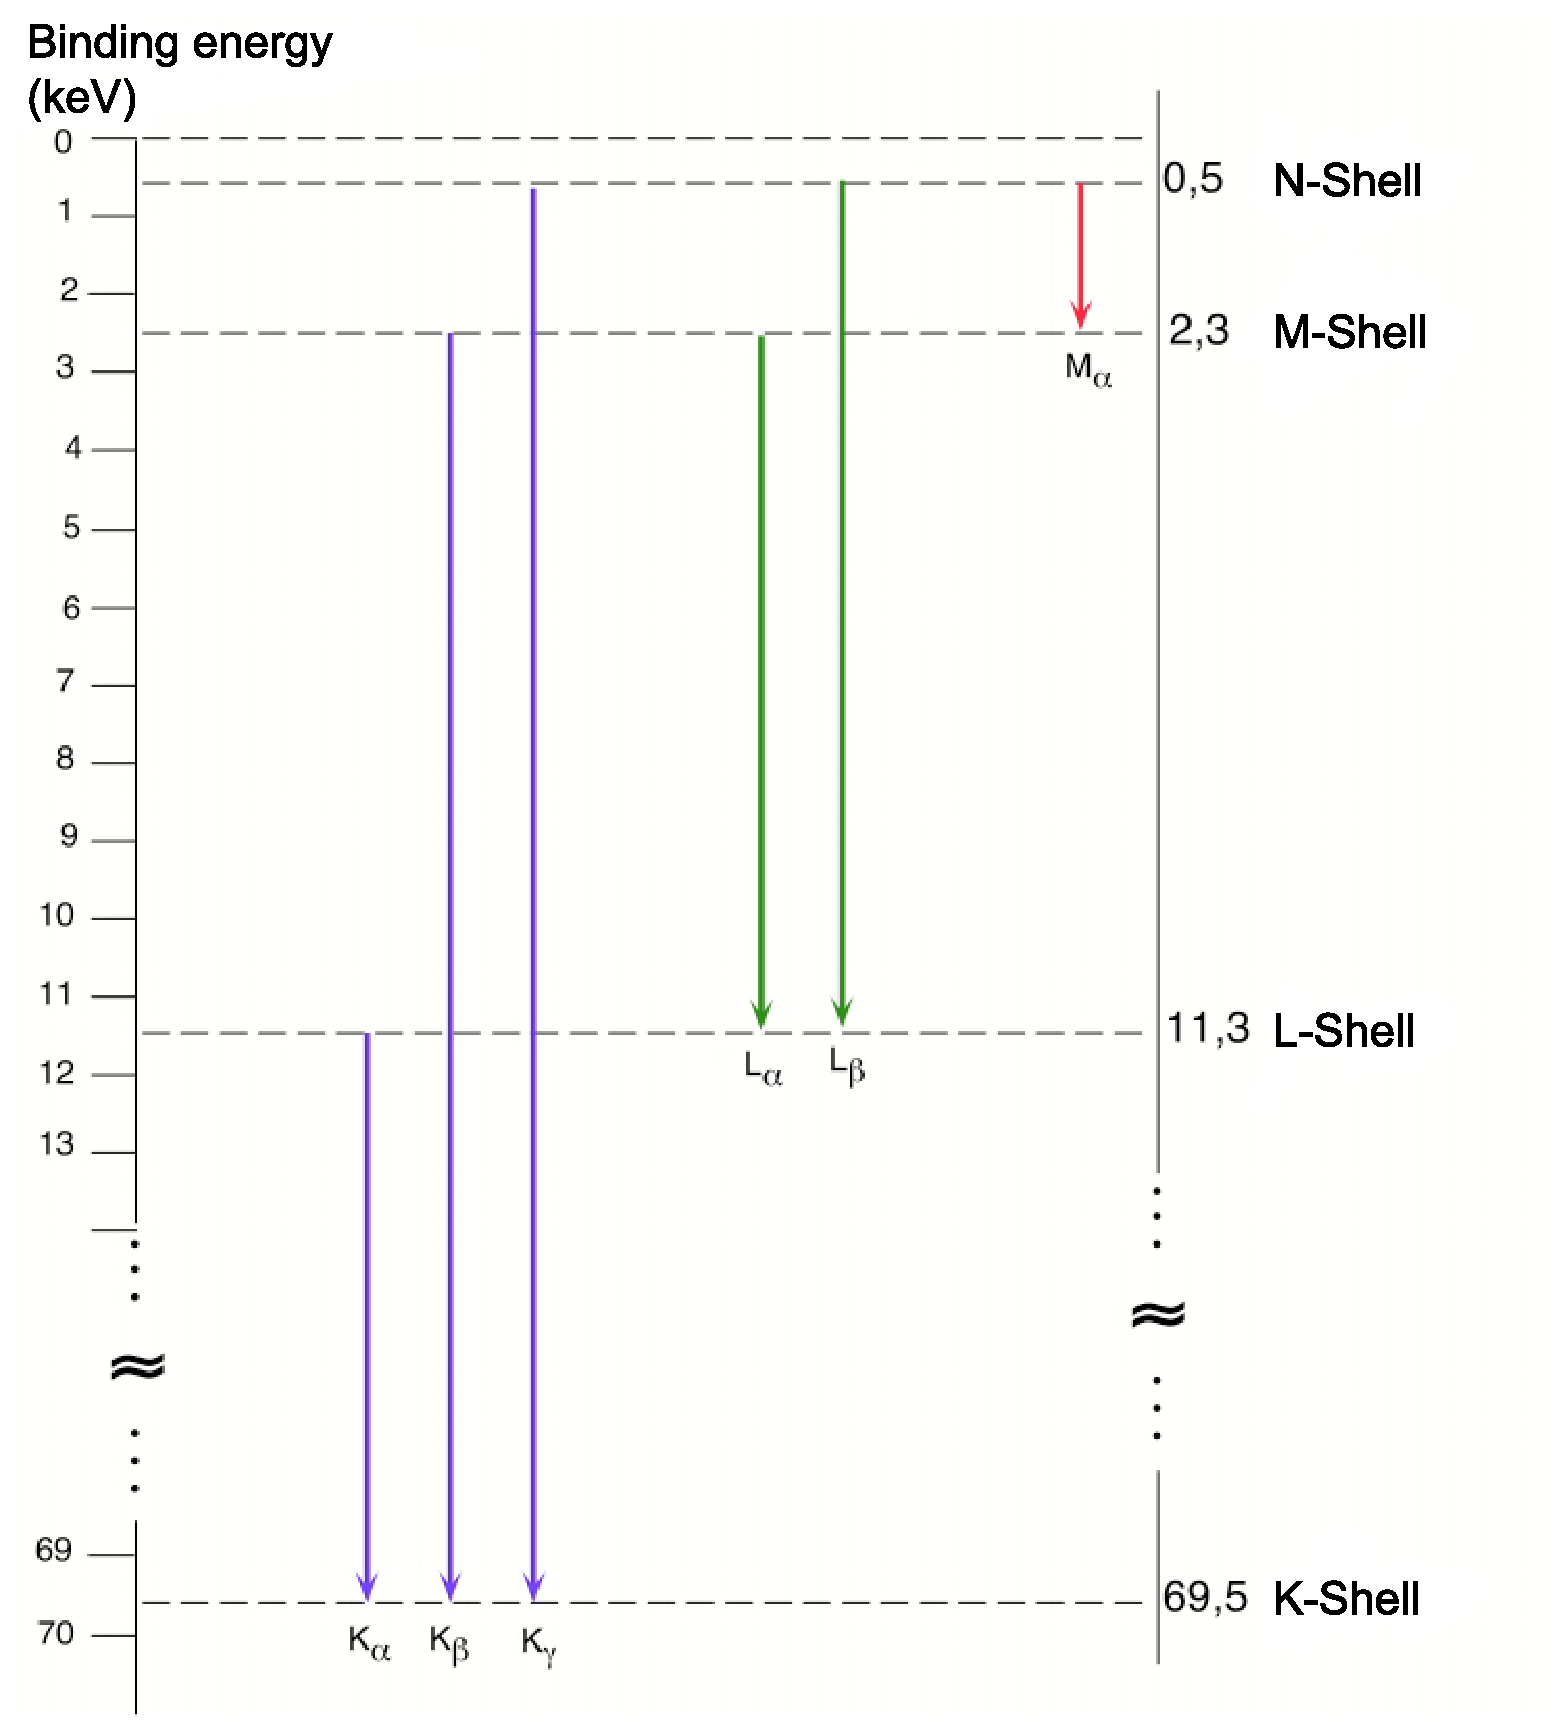
\includegraphics[height=0.8\textheight ]{images/tungsten_energylevel}\end{center}
    \begin{flushright}
        \scriptsize Source: Slides BVM
    \end{flushright}
\end{frame}

%%\begin{frame}{Overview of K-, L-, and M- Lines, \\and Absorption Edges}
%%\begin{columns}
%%\column{.5\textwidth}
%%Moseley's law:
%%\[
%%	\frac{1}{\lambda_{K_\alpha}}=R_{\infty} \cdot (Z-1) \cdot \frac{3}{4}
%%\]
%%\begin{table}[t]
%%	\centering
%%		\begin{tabular}{r l}
%%			$\lambda$  =& wavelength of $K_\alpha$-line \\
%%			$R_\infty$ =& Rydberg constant\\
%%			 ~&($10,973,731.6\ \textnormal{m}^{-1}$) \\
%% 			$Z$ =& atomic number
%%	\end{tabular}
%%\end{table}
%%\column{.5\textwidth}
%%\vspace{-0.2\textheight}\begin{center}\includegraphics[height=0.8\textheight ]{images/ch1a-20}\end{center}
%%\end{columns}
%%\begin{flushright}
%%\scriptsize Source: Slides BVM
%%\end{flushright}
%%\end{frame}

\begin{frame}{X-ray energy spectrum}
    \begin{itemize}
        \item When the electron reaches the anode, most of its energy is converted to heat energy (about 99\%!)
              \begin{itemize}
                  \item For example, 80 kVp tube voltage, 99.4\% is heat, 0.6\% is X-rays.
              \end{itemize}

    \end{itemize}
\end{frame}

\begin{frame}{Diagnostic X-Ray Tube Spectrum}
    \begin{center}\includegraphics[height=0.8\textheight ]{images/spectrum-diff-voltages}\end{center}
\end{frame}

\begin{frame}[c]{Energy Efficiency}
    \begin{eqnarray*}
        \eta&=&\frac{J_{total}}{I_A \cdot U_A}
    \end{eqnarray*}
    \begin{table}[t]
        \centering
        \begin{tabular}{r l}
            $J_{total}$ & = total X-ray power \\
            $I_A$       & = anode current     \\
            $U_A$       & = anode voltage     \\
        \end{tabular}
    \end{table}
\end{frame}

\begin{frame}[c]{Efficiency as Function of Atomic Number and Anode Voltage}
    \centering
    \begin{eqnarray*}
        \eta&=& k \cdot U_A \cdot Z\\
        ( k&\approx& 1 \cdot 10^{-9} V^{-1} )
        \label{eq:efficient}
    \end{eqnarray*}


    \vskip36pt
    \begin{itemize}
        \item Tungsten ($Z=74$), with $U_A=100 \text{ kV}$ $\Rightarrow$ $\eta=0.7 \ \%$
        \item Emitted X-ray power: 	$J_{total}=\eta\cdot I_A \cdot U_A$
    \end{itemize}
\end{frame}

\subtitle{X-Ray - Part 2}
\frame[plain,c]{\titlepage} % plain-Option deaktiviert Kopf- und Fusszeile



\section{X-ray and Matter Interaction}

%%%%%%%%%%%%%%%%%%%%%%%%%%%%%%%%%%%%%%%%%%%%%%%%%%%%%%%%%%%%%%%%%%%%%%%%%%

%%\begin{frame}{X-Ray Attenuation}
%%Suppose $I$ X-ray photons interact on a homogeneous material with thickness $x$.\\
%%When $x$ is a very small number, the expected number of photons $dI$ that interact and are removed from the X-ray beam can be written
%%in differential form:
%%\begin{center}
%%$dI=-\mu \cdot I \cdot dx $
%%\end{center}
%%\vskip12pt
%%\begin{table}[t]
%%	\centering
%%		\begin{tabular}{r l}
%%		\Large $I$ & =  \Large  number of incident X-ray photons \\
%%		\Large $dI$ & = \Large number of photons attenuated by material\\
%%		\Large $x$ & = \Large thickness of material \\
%%		\Large $\mu$ & = \Large linear attenuation coefficient (Unit of $\mu$: inverse length, e.g. $\textnormal{mm}^{-1}$	)\\
%%		\end{tabular}
%%\end{table}
%%\end{frame}
%%\begin{frame}{X-Ray Attenuation}
%%Conversion to integral form:
%%\vspace{-0.5cm}
%%\begin{eqnarray}
%%dI(x)&=&-\mu \cdot I(x) \cdot dx\nonumber \\
%%\frac{dI(x)}{I(x)}&=&-\mu \cdot dx \nonumber\\
%%\int_0^x \frac{1}{I(x)} dI(x) &=& - \int_0^x \mu dx\nonumber\\
%%  \log I(x)-\log I(0) &=& -\mu x\nonumber\\
%%  \log \frac{I(x)}{I(0)} &=& -\mu x\nonumber\\
%%  \frac{I(x)}{I(0)} &=& e^{-\mu x}\nonumber\\
%%  {I(x)} &=& I_0 e^{-\mu x}\nonumber
%%\end{eqnarray}
%%\end{frame}

\begin{frame}{X-Ray Attenuation}
    Define $I_0$ is the incident X-ray intensity. \\
    \vskip12pt
    \bluefat{Lambert-Beer's Law}: For a monoenergetic beam that passes through a homogeneous material with linear attenuation coefficient  $\mu$\\
    \begin{center}
        \vskip6pt
        $I=I_0\cdot e^{-\mu\cdot x}$\\
        $I=I_0\cdot e^{-\int\mu dx}$
    \end{center}

    In practical, emitted X-ray photons have various energies, resulting in polyenergetic energy spectra.
    The expected total number of photons after passing through the object is:
    \begin{center}
        $I = \int_{0}^{E_{\text{max}}}I_0(E) e^{ -\int{\mu dx} }dE$
    \end{center}

    % \vskip12pt
    % half value layer: $\frac{I}{I_0}=\frac{1}{2}=e^{-\mu \cdot d_{0.5}}$ \\ %
    % \vskip6pt
    % $\text{mass attenuation coefficient} = \frac{\mu}{\rho}$, \ with 
    % $\rho$ = density of material
\end{frame}

%\begin{frame}{Cross Section}
%\begin{columns}
%        \column{.35\textwidth}
%                \[ \sigma=\mu \cdot \frac{u A}{\rho} \]
%        \column{.65\textwidth}
%                \begin{table}[t]
%								\centering
%									\begin{tabular}{r l}
%									$\sigma$ & = cross section of an interaction \\ 
%									$\mu$ & = attenuation coefficient for an interaction \\
% 									$u$ & = atomic mass unit. $u = 1.6605402 \times 10^{-24} g$ \\
%									$A$ & = relative atomic mass of the target element \\
%									$\rho$ & = target element density\\
%									\end{tabular}
%							\end{table}
%\end{columns}
%\begin{columns}
%        \column{.3\textwidth}
%                \includegraphics[scale=.55]{images/cross-section}
%        \column{.6\textwidth}\vspace{-0.25\textheight}
%								\[ \frac{dN}{N}=-\mu\ dx = -\sigma \frac{\rho}{u A}\ dx \]
%\end{columns}\end{frame}

% \begin{frame}{Experimental Setup for Measuring the Attenuation Coefficient}
% \begin{center}\includegraphics[width=0.8\textwidth ]{images/ch1a-26}\end{center}
% \begin{flushright}
% \scriptsize Source: Slides BVM
% \end{flushright}
% \end{frame}

\begin{frame}{Interaction of X-Rays with Matter}
    \begin{eqnarray}
        \mu_\text{total} = \textcolor{red}{\mu_\text{pe} + \mu_{R} + \mu_{C}} + \mu_\text{pair} + \mu_\text{ph.n}
    \end{eqnarray}

    \begin{table}[t]
        \centering
        \begin{tabular}{r l}
            $\mu_\text{pe}$   & = attenuation coefficient for photoabsorption          \\
            %source: http://adsabs.harvard.edu/abs/1993ADNDT..54..181H
            $\mu_{R}$         & = attenuation coefficient for Rayleigh scattering      \\
            $\mu_{C}$         & = attenuation coefficient for Compton scattering       \\
            $\mu_\text{pair}$ & = attenuation coefficient for pair production          \\
            $\mu_\text{ph.n}$ & = attenuation coefficient for photon-nuclear reactions \\
            %source: http://www.uio.no/studier/emner/matnat/fys/FYS-KJM4710/v06/undervisningsmateriale/Photons2.pdf
        \end{tabular}
    \end{table}
\end{frame}

% \begin{frame}{Interaction of X-Rays with Matter}
% \begin{center}\includegraphics[height=0.8\textheight ]{images/interaction}\end{center}
% \end{frame}

\begin{frame}[c]{Photoelectric Absorption}
    \begin{columns}[c]
        \column{.45\textwidth}
        %\vspace{-0.5\textheight}
        \begin{itemize}
            \setlength\itemsep{0.2cm}
            \item Incident photon collides with an inner-shell electron in an atom of the absorbing material
            \item Incident photon ceases to exit
            \item The electron is ejected from its shell and becomes a recoil electron
                  \begin{itemize}
                      \item[$\Rightarrow$] \bluefat{Photoelectron}
                  \end{itemize}
        \end{itemize}
        \column{.45\textwidth}
        \includegraphics[height=0.6\textheight]{images/pe}\\[-0.5\baselineskip]
    \end{columns}
\end{frame}

\begin{frame}[c]{Compton Scattering}
    \begin{columns}[c]
        \column{.45\textwidth}
        %\vspace{-0.55\textheight}
        \begin{itemize}
            \setlength\itemsep{0.2cm}
            \item Incident photon interacts with an outer orbital electron
            \item Incident photon with lower energy is deflected and scattered from the atom
            \item Almost all scattered radiation in diagnostic radiology comes from Compton scattering
        \end{itemize}
        \column{.45\textwidth}
        \includegraphics[height=0.6\textheight]{images/compton}\\[-0.5\baselineskip]
    \end{columns}
\end{frame}

\begin{frame}[c]{Rayleigh Scattering}
    \begin{columns}[c]
        \column{.45\textwidth}
        %\vspace{-0.5\textheight}
        \begin{itemize}
            \setlength\itemsep{0.2cm}
            \item Low energy incident photon interacts with the outer-shell electron
            \item Electron is set into vibration, which emits radiation
            \item The direction of the incident Photon is altered
            \item Contributes very little in diagnostic radiology
        \end{itemize}
        \column{.45\textwidth}
        \includegraphics[height=0.5\textheight]{images/rayleigh}\\[-0.5\baselineskip]
    \end{columns}
    % \begin{center}\includegraphics[height=0.8\textheight ]{images/pe}\end{center}
\end{frame}


% \begin{frame}{Energy Transformation Coefficients}
% \begin{center}\includegraphics[height=0.8\textheight ]{images/ch1a-29}\end{center}
% \begin{flushright}
% \scriptsize Source: Slides BVM
% \end{flushright}
% \end{frame}


\begin{frame}[c]{Mass Attenuation Coefficient for Iron}
    \begin{figure}[c]
        \centering
        \tiny	\def\svgwidth{0.65\textwidth}
        \input{Attenuation_Coefficient_Iron.pdf_tex}

        %\caption{}
        %\label{fig:}
    \end{figure}
    \vspace{-1cm}
    \begin{flushright}
        \tiny Source: Jarekt (CC BY-SA 3.0)
    \end{flushright}
\end{frame}

\begin{frame}{Mass Attenuation Coefficient for Lead}
    \begin{columns}[c, onlytextwidth]
        \begin{column}{0.5\textwidth}
            \begin{center}\includegraphics[height=0.8\textheight, trim={2cm  3.5cm 2cm 2cm},clip ]{images/lead_attenuation_mit_opencourse_ware.jpg}\end{center}
        \end{column}\begin{column}{0.5\textwidth}
            \begin{itemize}
                \item[$ \frac{\tau}{\rho}$] Attenuation due to photoelectric effect
                \item[$ \frac{\sigma}{\rho}$] Compton effect
                \item[$ \frac{\sigma_R}{\rho}$] Rayleigh scattering
                \item[$ \frac{\kappa}{\rho}$] Pair production
                \item[$ \frac{\mu}{\rho}$] Total attenuation

            \end{itemize}

        \end{column}
    \end{columns}
\end{frame}


\begin{frame}{Mass Attenuation Coefficient for Water}
    \begin{center}\includegraphics[height=0.8\textheight ]{images/Mass-attenuation-coefficients-for-photons-in-water-source-MIT-OpenCourseWare-22101.png}\end{center}
    \begin{flushright}
        \tiny Source: MIT OpenCourseWare (CC BY-NC-SA 2.0 )
    \end{flushright}
\end{frame}


%\begin{frame}{Mass Attenuation Coefficient for Lead}
%\begin{center}\includegraphics[height=0.8\textheight ]{images/lead}\end{center}
%\end{frame}

%\begin{frame}{Mass Attenuation Coefficient for Water}
%\begin{center}\includegraphics[height=0.8\textheight ]{images/water}\end{center}
%\end{frame}

% \begin{frame}{Summary of Attenuation Factors}
% \begin{center}
% 	\begin{tabular}{p{5cm}|p{5cm}|p{5cm}|p{5cm}}
% 		wavelength & atomic number & mass density & thickness \\
% 		\hline
% 		\begin{center}\includegraphics[scale=.2]{images/atten-1}\end{center} & \begin{center}\includegraphics[scale=.2]{images/atten-2}\end{center}&\begin{center}\includegraphics[scale=.2]{images/atten-3}\end{center}&\begin{center}\includegraphics[scale=.2]{images/atten-4}\end{center}\\
% 		\hline
% 		attenuation proportional to the 3. potent of wavelength & attenuation proportional to the 3. potent of atomic number & attenuation proportional to the density & attenuation proportional to thickness
% 			\end{tabular}
% \end{center}
% \begin{flushright}
% \scriptsize Source: BVM
% \end{flushright}
% \end{frame}


%%%%%%%%%%%%%%%%%%%%%%%%%%%%%%%%%%%%%%%%%%%%%%%%%%%%%%%%%%%%%%%%%%%%%%%

\subtitle{X-Ray - Part 3}
\frame[plain,c]{\titlepage} % plain-Option deaktiviert Kopf- und Fusszeile


\section{X-ray Imaging}

\begin{frame}{Definition}
    \begin{tabular}{lccl}
        X-ray Generation          & {$\longrightarrow$}          &  & Conversion of electrons to X-rays       \\
        X-ray Matter Interacation & {$\longrightarrow$}          &  & Attenuation of X-rays                   \\
        \textbf{X-ray Imaging}    & \textbf{{$\longrightarrow$}} &  & \textbf{Conversion of X-rays to images}
    \end{tabular}\\
    \vspace{2cm}
    \textbf{We will discuss:}
    \begin{itemize}
        \item Image intensifier systems
        \item Flat panel detectors
        \item Sources of noise in X-ray imaging
    \end{itemize}
\end{frame}

\begin{frame}{Image Intensifiers}
    \begin{itemize}
        \item Image intensifier are vacuum tubes that convert X-rays to visible light
        \item Light intensity can be adjusted by electron optics
        \item Image can then be viewed directly at an output screen
        \item First introduced in the late 1940's for fluroscopy applications
    \end{itemize}
    \vspace{0.25cm}
    \begin{center}
        \includegraphics[width=0.3\textwidth]{images/ImageIntensifierSiemens2}\hspace{2cm}
        \includegraphics[width=0.3\textwidth]{images/ImageIntensifierSiemens}
    \end{center}
    \begin{flushright}
        \scriptsize Sources: Siemens Healthcare, Erlangen, Germany
    \end{flushright}
\end{frame}

\begin{frame}{Image Intensifiers - Function}
    \begin{center}
        \includegraphics[width=0.95\textwidth]{images/Intensifier_Schematic}
    \end{center}
    \begin{enumerate}
        \item X-rays are converted to light by scintillator material (Input Phosphor)
        \item Light photons are converted to electrons using a photocathode
        \item Electrons are accelerated and focused by an electron optics
        \item Fast electrons are converted to light when they hit the output phosphor, which yields the output image.
        \item Image is typically captured by a camera and transferred to a monitor
    \end{enumerate}
\end{frame}

\begin{frame}{Image Intensifiers -- Detailed Function}
    \begin{center}
        \includegraphics[width=0.8\textwidth]{images/Intensifier_Detail}
    \end{center}
\end{frame}

\begin{frame}{Scintillator -- Input Phosphor}
    \begin{itemize}
        \setlength\itemsep{0.3cm}
        \item  Only absorbed X-ray photons can be converted to light\\
              $\rightarrow$ Scintillator material should have high attenuation coefficients for\\ \hspace{1cm}energies of typical X-ray spectra
        \item  Light should exit the scintillator at position of absorption to preserve spatial resolution\\
              $\rightarrow$ Scattering of light photons inside material should be low
        \item  Produced light photon's wavelength should match the photocathode
        \item  Typical scintillator materials are
              \begin{itemize}
                  \item zinc-cadmium sulfide (ZnCdS)% / used since the early years of image intensifiers
                  \item cesium-iodide (CsI)% / newer material with improved properties
              \end{itemize}
    \end{itemize}
\end{frame}

\begin{frame}{ZnCdS vs. CsI - Attenuation and Light Photon Wavelength}
    \begin{figure}[tb]%
        \centering
        \begin{minipage}[c]{0.47\columnwidth}
            \includegraphics[width=1\columnwidth]{images/AbsorptionPhosphorMaterial}%
            \caption{Mass attenuation coefficient of CsI and ZnCdS and the estimated X-ray spectrum after transmission through the patient.}
        \end{minipage}
        \hspace{0.5cm}
        \begin{minipage}[c]{0.47\columnwidth}
            \includegraphics[width=1\columnwidth]{images/SensitivityPhosphorPhotocathode}%
            \caption{Sensitivity of an SbCs$_3$ photocathode and characteristic light spectra emitted from a CsI as well as a ZnCdS phospor layer.}
        \end{minipage}%
    \end{figure}
\end{frame}

\begin{frame}{ZnCdS vs. CsI - Spatial Resolution}
    \begin{itemize}
        \item  CsI can be manufactured with tubular structure
        \item  Tubes act as optical-fibre and prevent scattering of light
        \item  Produced light can be better assigned to incoming X-ray location
    \end{itemize}
    \begin{center}
        \hspace{-2cm}\includegraphics[width=0.75\columnwidth]{images/CsI_structure}%
    \end{center}
\end{frame}

\begin{frame}{Image Intensifiers -- Known Problems}
    \begin{itemize}
        \item  Small changes in external magnetic or electric field can change electron trajectories in electron optics $\rightarrow$ Image distortion
        \item  Light scattering in output phosphor is isotropic
        \item  However, no scattering contribution from outside the material to periphery $\rightarrow$ Vignetting effect
    \end{itemize}
    \vspace{-0.4cm}
    \begin{figure}[tb]%
        \centering
        \begin{minipage}[t]{0.448\columnwidth}
            \includegraphics[width=1\columnwidth]{images/Vignetting}\vspace{-0.2cm}%
            \caption{Vignetting artifact: Luminescence drops at image periphery.}
        \end{minipage}
        \hspace{0.06\columnwidth}
        \begin{minipage}[t]{0.272\columnwidth}
            \includegraphics[width=0.85\columnwidth]{images/Distortion}\vspace{-0cm}%
            \caption{Distortion due to electric or magnetic field.}
        \end{minipage}%
    \end{figure}
\end{frame}

\begin{frame}{Flat Panel Detectors}
    \begin{itemize}
        \item Flat Panel Detectors (FPD) digitize image data directly
        \item There exist direct and indirect FPDs
              \begin{itemize}
                  \item Direct $\rightarrow$ Converts X-rays directly to electrical charges
                  \item Indirect $\rightarrow$ Converts X-rays to light and then to electrical charge
              \end{itemize}
        \item Images can be easily viewed, shared, stored, etc.
        \item First introduced in the mid 1990s
        \item Suitable for radiography, fluroscopy and cone-beam CT
    \end{itemize}
    \vspace{0.25cm}
    \begin{center}
        \includegraphics[width=0.25\textwidth]{images/FlatPanelSiemens}\hspace{2cm}
        \includegraphics[width=0.25\textwidth]{images/FlatPanelSiemens2}
    \end{center}
    \begin{flushright}
        \scriptsize Sources: Siemens Healthcare, Erlangen, Germany
    \end{flushright}
\end{frame}


\begin{frame}[c]{FPD -- Direct Conversion}
    \begin{enumerate}
        \setlength\itemsep{0.3cm}
        \item X-ray sensitive photoconducter absorbs X-rays
        \item X-ray absorption causes electron-hole pairs
        \item Global electric field $E_{ph}$: Anode at top and Cathode at bottom
        \item In each pixel cell the positive charges travel to the bottom and are stored locally in capacitors
    \end{enumerate}
    %\vspace{-0.5cm}
    %\begin{center}
    %\includegraphics[width=0.47\columnwidth]{images/directFPD}%
    %\end{center}
\end{frame}

\begin{frame}{FPD -- Indirect Conversion}
    \begin{enumerate}
        \item Scintillator material (CsI) converts X-rays to light photons
        \item Dense matrix of photodiodes (pixels) convert light to electrical charge
        \item Electrical charge is stored locally in each pixel's capacitor
    \end{enumerate}
    \vspace{-0cm}
    \begin{center}
        \includegraphics[height=0.6\textheight]{images/FlatDetectorSystem}%
    \end{center}
\end{frame}

\begin{frame}{FPD -- Data Readout (Direct and Indirect)}
    \begin{itemize}
        \vspace{0.2cm}
        \item After a certain time of radiation exposure each pixel will have charges in its storage capacitor
        \item Read-out is done row-wise with a certain read-out frequency
        \item Row is selected by switching on the Thin-Foil Transistors (TFT) of this row's pixels
        \item Stored charges in pixels are directed to a charge integrating amplifier
        \item After amplifier the datastream is digitized (analog-to-digital-conversion)
        \item Data is directly sent to a computer system over a bus
        \item Pixels can be combined (binning) to increase read-out speed and SNR
    \end{itemize}
\end{frame}

\begin{frame}{Sources of Noise}
    \begin{itemize}
        \vspace{0.3cm}
        \item Two types of undesired effects in X-ray imaging
              \begin{itemize}
                  \item Image noise
                  \item Image artifacts
              \end{itemize}
        \item Both based on physical effects
        \item Difference: When scan is repeated with identical settings,
              \begin{itemize}
                  \item artifacts (e.g., aliasing) will remain unchanged
                  \item noise pattern will vary as it is a probabilistic effect
              \end{itemize}
        \item Prerequisites: Discrete statistical distributions
              \begin{itemize}
                  \item Poisson distribution
                  \item Binomial distribution
              \end{itemize}
    \end{itemize}
\end{frame}

\begin{frame}{Poisson distribution}

    \begin{columns}[c, onlytextwidth]
        \begin{column}{0.4\textwidth}
            \begin{itemize}
                \item Poisson distribution is discrete distribution with density function:
                      \begin{equation*}
                          p(\mathcal{N}=n)=\frac{(N_{_0})^n}{n!}\,e^{-N_{_0}}
                      \end{equation*}
                \item $N_{_0}$ is the expectation value and only parameter
                \item Comparable to a normal distribution for large $N_{_0}$
            \end{itemize}
        \end{column}\begin{column}{0.6\textwidth}
            \begin{center}
                \includegraphics[height=0.7\textheight]{images/PoissoinVsGauss}%
            \end{center}
        \end{column}
    \end{columns}
\end{frame}

\begin{frame}{Poisson distribution - Example}
    \begin{itemize}
        \item Local shop writes down number of customers per day for one year
        \item The average number of customers per day is $N_{_0}=15$
        \item What is probability that tomorrow will be $n=20$ customers in the shop
              \begin{eqnarray}
                  p(\mathcal{N}=20) &=& \frac{(N_{_0})^n}{n!}\,e^{-N_{_0}}\nonumber\\[0.5cm]
                  &=&  \frac{15^{20}}{20!}\,e^{-15} \nonumber\\[0.5cm]
                  &\approx& 0.0418 \nonumber
                  \label{eq:sdf}
              \end{eqnarray}
        \item Probability that tomorrow will be $n=20$ customers there is 4.18\%
    \end{itemize}
\end{frame}

\begin{frame}{Binomial distribution}
    \begin{itemize}
        \item Used for a series of independent random experiments with binary outcome, e.g., ``yes or no'' or ``heads or tails''
              \begin{equation*}
                  p(\mathcal{N}=n)=\binom{N}{n}\,p^n\,(1-p)^{N-n} = \frac{N!}{n!\,(N-n)!}\,p^n\,(1-p)^{N-n}
              \end{equation*}
        \item Probability that exactly $n$ positive outcomes occur for $N$ independent trials
        \item $p$ is the probability that a single trial has a positive outcome
    \end{itemize}\vspace{0cm}
    \begin{center}
        \includegraphics[width=0.3\columnwidth]{images/Binomi}%
    \end{center}
\end{frame}

\begin{frame}{Binomial distribution - Example}
    \begin{itemize}
        \item Probability that coin shows $n=20$ times heads if tossed $N=30$ times
        \item If coin is ideal the chance is ``fifty-fifty'', i.e., $p=0.5$
              \begin{eqnarray}
                  p(\mathcal{N}=20) &=& \binom{N}{n}\,p^n\,(1-p)^{N-n}\nonumber\\[0.4cm]
                  &=&\frac{30!}{20!\,(30-20)!}\,(0.5)^{20}\,(1-0.5)^{30-20}\nonumber\\[0.5cm]
                  &\approx& 0.028\nonumber
                  \label{eq:sdf2}
              \end{eqnarray}
        \item Probability of 20 times heads for 30 times coin tossing is 2.8\%
    \end{itemize}
\end{frame}

\begin{frame}{Sources of Noise}
    \begin{center}
        \includegraphics[width=1\textwidth]{images/NoiseOverview}
    \end{center}
    \begin{itemize}
        \item Different statistical processes occur at the different states of an X-ray imaging system
        \item Conversion from electrons to X-rays follows Poisson distribution
        \item Each generated x-ray photon interacts independent of the others, thus, all following steps follow binomial distributions
    \end{itemize}
\end{frame}

\begin{frame}{Statistics of the X-ray Generation Process}
    \begin{itemize}
        \item Number of generated X-ray photons at anode is Poisson distributed
        \item $N_e$ is the number of accelerated fast electrons
        \item $p_{ex}$ is probability that a fast electron triggers an X-ray photon
        \item The probability that the source produces $n$ photons is then given by
              \vspace{0.5cm}
              \begin{eqnarray}
                  P(\mathcal{N}=n) &=& \frac{N_{_0}}{n!}\,e^{-N_{_0}}\nonumber\\[0.5cm]
                  &=& \frac{N_e\,p_{ex}}{n!}\,e^{-N_e\,p_{ex}}\nonumber
              \end{eqnarray}
              \vspace{0.01cm}
        \item Where the expectation value is given with $N_{_0}=N_e\,p_{ex}$
              %\item Definition: $P(N_x)$ is the probability that the source produces $N_x$ photons 
    \end{itemize}
\end{frame}

\begin{frame}{Statistics of the X-ray Matter Interaction}
    \begin{itemize}
        \item Generated X-ray photons interact with matter
        \item Photons either absorbed or unaffected $\rightarrow$ Binomial distribution
        \item Probability $p_a$ for a photon passing unaffected is given by Beer's law
              \begin{equation*}
                  p_a = e^{-\int \mu(s) ds}
              \end{equation*}
        \item The probability that $n_s$ photons pass unaffected \textbf{and} that $N_x$ photons have been produced is called the \textbf{Joint Probability} $P(n_s,N_x)$
              %\item From Bayes law we get:
              %\begin{equation*}
              %P(n_s,N_x) = P(N_x) \times P(n_s|N_x)
              %\end{equation*}
              %\item Using marginalisation (``Law of Total Probability'') we get:
              %\begin{equation*}
              %P(n_s,N_x) = P(N_x) \times P(n_s|N_x)
              %\end{equation*}
    \end{itemize}
\end{frame}

%\begin{frame}{Statistics of the X-ray Matter Interaction}
%	\begin{itemize}
%		\item We are interested in the probability that $n_s$ photons passed the object
%		\item To compute $P(N = n_s)$ we need to apply marginalisation
%			\begin{eqnarray}
%				P(N = n_s) &=& \sum_{N_x=n_s}^\infty \,\, P(n_s,N_x) \nonumber\\
%									 &=& \sum_{N_x=n_s}^\infty \,\, P(N_x) \times P(n_s|N_x) \nonumber\\
%									 &=& \sum_{N_x=n_s}^\infty \,\, \underbrace{\frac{(N_{_0})^{N_x}}{N_x!}\,e^{-N_{_0}}}_\text{Prob. $N_x$ photons generated}  \times \underbrace{\binom{N_x}{n_s}\,p_a^{n_s}\,(1-p_a)^{N_x-n_s}}_\text{Prob. that $n_s$ of $N_x$ photons pass}\nonumber
%			\end{eqnarray}
%	\end{itemize}
%\end{frame}
%
%\begin{frame}{Statistics of the X-ray Matter Interaction}
%	\begin{itemize}
%		\item It can be shown that the marginalisation evaluates to\footnote{We refer to the book of Buzug ``Computed Tomography: From Photon Statistics to Modern Cone-Beam CT'' page 65 for a detailed derivation}
%			\begin{eqnarray}
%				P(N = n_s)  &=& \sum_{N_x=n_s}^\infty \,\, \frac{(N_{_0})^{N_x}}{N_x!}\,e^{-N_{_0}} \times \binom{N_x}{n_s}\,p_a^{n_s}\,(1-p_a)^{N_x-n_s}\nonumber\\
%					&=& \frac{( N_{_0} \,p_a)^{n_s}}{n_s!}\,e^{-N_{_0}p_a} \nonumber
%			\end{eqnarray}
%			\item Result: $P(N = n_s)$ is again a Poisson distribution!
%			\item The expectation value is again Beer's law
%			\begin{equation*}
%				E(\mathcal{N}) = N_{_0} p_a = N_{_0} e^{-\int \mu(s) ds}
%			\end{equation*}
%	\end{itemize}
%\end{frame}

\begin{frame}{SNR and Noise}
    \begin{itemize}
        \item The signal-to-noise ratio (SNR) can also be defined by statistics
              \begin{equation*}
                  SNR(\mathcal{N}) =  \frac{\mu}{\sigma} = \frac{E(\mathcal{N})}{\sqrt{E((\mathcal{N}-\mu)^2)}}
              \end{equation*}
        \item $\mu$ is the expectation value of $\mathcal{N}$ $\rightarrow$ Measure for signal strength
        \item $\sigma$ is the square root of the variance of $\mathcal{N}$ $\rightarrow$ Measure for noise
        \item SNR increases if the signal strength increases or if the noise reduces
    \end{itemize}
\end{frame}

\begin{frame}{SNR and Noise}
    \begin{itemize}
        \item For Poisson the expectation value equals the variance, thus $\mu = \sigma^2$
        \item Hence, $\mu = N_{_0} p_a$ and $\sigma = \sqrt{N_{_0} p_a}$
        \item The SNR after the X-rays pass through the patient computes to
              \vspace{0.25cm}
              \begin{eqnarray}
                  SNR(\mathcal{N}) &=& \frac{N_{_0}\,p_a}{\sqrt{N_{_0}\,p_a}} \nonumber\\[0.25cm]
                  &=& \sqrt{N_{_0} \,p_a} \nonumber\\[0.25cm]
                  &=& \sqrt{N_{_0}} \,\, e^{-\frac{1}{2}\int \mu(s) ds} \nonumber
              \end{eqnarray}
        \item SNR increases with the square root of the number of input photons
        \item High mass attenuation $\mu(s)$ or thick materials decrease the SNR
    \end{itemize}
\end{frame}

\section{Applications of X-Rays}

\begin{frame}{Radiography}
    \begin{itemize}
        \item Two dimensional X-ray projection images
        \item Object is exposed to X-rays and attenuation of the object is measured
        \item Main application: Examination of fractures or changes of skeletal system
        \item Bones attenuate more than surrounding tissue $\rightarrow$ Good contrast
              \vspace{0.3cm}
    \end{itemize}
    \begin{center}
        \hfill{}\includegraphics[width=0.65\textwidth]{images/Broken_fixed_arm}\hfill{} \scriptsize Sources: Wikimedia / Public Domain
    \end{center}
\end{frame}

\begin{frame}[c]{Fluroscopy}
    \begin{itemize}
        \setlength\itemsep{0.4cm}
        \item Sequence of radiography images with certain framerate
        \item X-ray source either triggered or constant radiation
        \item Framerate is typically limited by acquisition speed of detector
              \begin{itemize}
                  \item Image Intensifier: Inertia of final fluorescent screen
                  \item FPDs: Electronic detector readout step
              \end{itemize}
        \item Important for minimally invasive interventions $\rightarrow$ catheters, endoscopes or other tools can be tracked over time
        \item Also key technology for digital subtraction angiography
    \end{itemize}
\end{frame}

\begin{frame}{Fluroscopy}
    %
    \begin{columns}[t, onlytextwidth]
        \begin{column}{0.4\textwidth}
            \begin{figure}[htpb]
                \centering
            \includegraphics[height=0.6\textheight]{images/Fluoroscopy_pacemaker_leads_right_atrium_ventricle}%
            \caption{Image of fluoroscopy sequence showing the placement of two electrodes of a pacemaker.}%
            \end{figure}
        \end{column}$\quad$\begin{column}{0.6\textwidth}
        \begin{figure}
            \centering
            \includegraphics[height=0.6\textheight]{Siemens_Images/SH_AX_36710_13}%
            \caption{Typical clinical setup of a minimally invasive surgery with a C-arm device. X-ray source at the bottom and the FPD is right above the patient.}%
        \end{figure}
        \end{column}
    \end{columns}
    %%
    \begin{flushright}
        \scriptsize Sources: Steven Fruitsmaak, Wikimedia Commons / Siemens Healthcare, Erlangen, Germany
    \end{flushright}
\end{frame}



\begin{frame}{Digital Subtraction Angiography --- Contrast Agent}
    \begin{itemize}
        \item Angiography = Imaging of arteries to analyze shape, size, lumen, etc.
        \item {\Huge \Lightning} Attenuation of vessels not much different to surrounding tissue {\Huge \Lightning}
        \item Contrast agent: Liquid with substantially higher attenuation coefficient than background material
        \item Contrast agent injected into vascular system to improve vessel contrast
        \item Typical contrast agent media are iodine and barium
        \item Iodine: Used for intravascular injections
        \item Barium: Stomach or colone examinations (Can be swallowed)
    \end{itemize}
\end{frame}

\begin{frame}{Digital Subtraction Angiography --- Principle}
    \begin{itemize}
        \item Fluroscopic sequence of fixed anatomy over time
        \item Simultaneous injection of contrast agent into arteries
        \item X-rays without contrast = Background tissue
        \item Subtract non-contrasted reference image from contrasted images
        \item Subtraction will result in image of contrasted arteries only
        \item Non-contrasted image = ``mask image''
        \item Contrasted images = ``fill images''
    \end{itemize}
\end{frame}

\begin{frame}[c]{Digital Subtraction Angiography --- Example}
    \begin{figure}[tb]%
        \centering
        \begin{tabular}{ccc}
            \includegraphics[height=.3\linewidth]{images/dsa_mask.pdf} & \includegraphics[height=.3\linewidth]{images/dsa_fill.pdf} & \includegraphics[height=.3\linewidth]{images/dsa_diff.pdf} \\
            {\color{faublue}(a) Mask image}                                               & {\color{faublue}(b) Fill image}                                               & {\color{faublue}{(c) Angiogram}}                                              \\
        \end{tabular}
        %\begin{columns}[t, onlytextwidth]
        %\begin{column}{0.3\textwidth}
        %\begin{figure}[]
        %\centering
        %\includegraphics[height=\linewidth]{../mt1-script/xray/images/dsa_mask.pdf}
        %\caption{Mask image}
        %\end{figure}
        %\end{column}\begin{column}{0.3\textwidth}
        %\begin{figure}[]
        %\centering
        %\includegraphics[height=\linewidth]{../mt1-script/xray/images/dsa_fill.pdf}
        %\caption{Fill image}
        %\end{figure}
        %\end{column}\begin{column}{0.3\textwidth}
        %\begin{figure}[]
        %\centering
        %\includegraphics[height=\linewidth]{../mt1-script/xray/images/dsa_diff.pdf}
        %\caption{Fill image}
        %\end{figure}
        %\end{column}
        %\end{columns}
        %\hspace*{.8cm}  \tiny Bildquelle: Adam Galant, Siemens Healtcare
        \caption{Process of creating a DSA. In (a) the hand was imaged and no contrast agent has been injected (mask image). In (b) the same hand has been imaged but including injected contrast agent. The difference of (a) and (b) represents the angiogram as shown in Figure (c).}\label{fig_chap:xray_dsa}
    \end{figure}
    \begin{flushright}
        \tiny Source: Adam Galant, Siemens Healthcare, Erlangen, Germany.
    \end{flushright}
\end{frame}



\section{Further Questions?}

\begin{frame}[t]{Further Readings}
    \begin{itemize}
        \item \fullcite{Berger2018}
    \end{itemize}

\end{frame}

\end{document}
